\documentclass[crop, tikz]{standalone}
\usepackage{tikz}

\usetikzlibrary{arrows,shapes, decorations.pathmorphing,backgrounds,positioning}
\usetikzlibrary{decorations.pathreplacing}
\usetikzlibrary{arrows.meta, calc}

\tikzstyle{latSmallNode}=[draw, circle, inner sep=2pt]
\tikzstyle{latStateTransition}=[->, thick, -{Latex[length=2mm,width=2mm]}]
\tikzstyle{cnSmallNode}=[draw, circle, inner sep=2pt]
\tikzstyle{invisNode}=[inner sep=2pt]
\tikzstyle{cnStateTransition}=[thick, ->, -{Latex[length=3mm,width=3mm]}, align=center]
\tikzstyle{matchingArc}=[thick, <->, align=center, color=purple]

\begin{document}
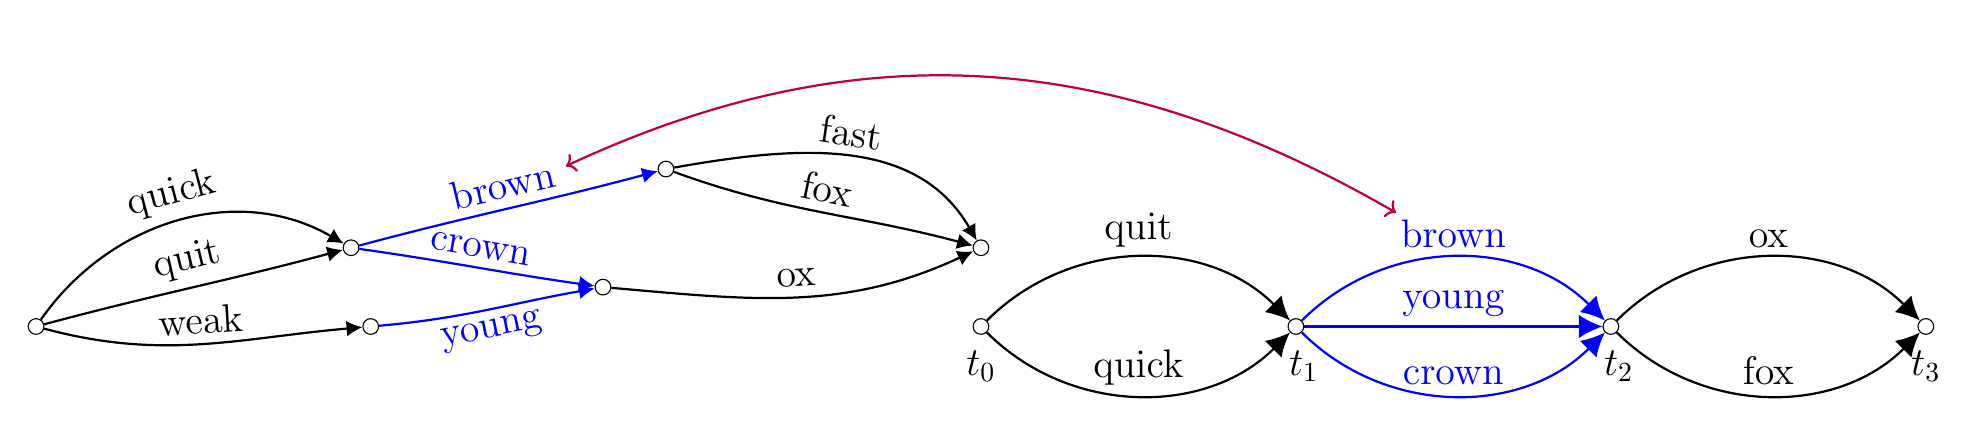
\begin{tikzpicture}
    % Lattice Nodes
    \node[latSmallNode] (latN1) at (0, 0) {};
    \node[latSmallNode] (latN2) at (0.25, -1) {};
    \node[latSmallNode] (latN3) at (4, 1) {};
    \node[latSmallNode] (latN4) at (3.2, -0.5) {};
    \node[latSmallNode] (latN5) at (8, 0) {};
    \node[latSmallNode] (latN6) at (-4, -1) {};
    
    % Lattice Arcs
    \draw[latStateTransition] (latN6) to[out=15,in=195] node [midway, sloped, above] {\Large{quit}} (latN1);
    \draw[latStateTransition] (latN6) to[out=55,in=150] node [midway, sloped, above] {\Large{quick}} (latN1);
    \draw[latStateTransition] (latN6) to[out=-15,in=185] node [midway, sloped, above] {\Large{weak}} (latN2);
    \draw[latStateTransition, color=blue] (latN1) to[out=352,in=172] node [midway, sloped, above] {\Large{crown}} (latN4);
    \draw[latStateTransition] (latN3) to[out=-20,in=165] node [midway, sloped, above] {\Large{fox}} (latN5);
    \draw[latStateTransition] (latN4) to[out=-5,in=205] node [midway, sloped, above] {\Large{ox}} (latN5);
    \draw[latStateTransition] (latN3) to[out=10,in=120] node [midway, sloped, above] {\Large{fast}} (latN5);
    \draw[latStateTransition, color=blue] (latN1) to[out=15,in=195] node [midway, sloped, above] {\Large{brown}} (latN3);
    \draw[latStateTransition, color=blue] (latN2) to[out=5,in=190] node [midway, sloped, below] {\Large{young}} (latN4);

    % Confusion Network Nodes
    \node[cnSmallNode] (n1) at (8, -1) {};
    \node[invisNode] (t1) at (8, -1.5) {\Large{$t_0$}};
    \node[cnSmallNode] (n2) at (12, -1) {};
    \node[invisNode] (t2) at (12.1, -1.5) {\Large{$t_1$}};
    \node[cnSmallNode] (n3) at (16, -1) {};
    \node[invisNode] (t3) at (16.1, -1.5) {\Large{$t_2$}};
    \node[cnSmallNode] (n4) at (20, -1) {};
    \node[invisNode] (t4) at (20, -1.5) {\Large{$t_3$}};

    % Confusion Network Arcs
    % 1-Best Path
	\draw[cnStateTransition] (n1) to[out=-45,in=-135] node [midway, sloped, above] {\Large{quick}} (n2);
	\draw[cnStateTransition, color=blue] (n2) to[out=0,in=180] node [midway, sloped, above] {\Large{young}} (n3);
	\draw[cnStateTransition] (n3) to[out=-45,in=-135] node [midway, sloped, above] {\Large{fox}} (n4);
	% Alternative Arcs
	\draw[cnStateTransition] (n1) to[out=45,in=135] node [midway, sloped, above] {\Large{quit}} (n2);
	\draw[cnStateTransition, color=blue] (n2) to[out=45,in=135] node [midway, sloped, above] {\Large{brown}} (n3);
	\draw[cnStateTransition] (n3) to[out=45,in=135] node [midway, sloped, above] {\Large{ox}} (n4);
 	\draw[cnStateTransition, color=blue] (n2) to[out=-45,in=-135] node [midway, sloped, above] {\Large{crown}} (n3);
 	
 	% Matching arcs
    \node[invisNode] (latTarget) at (2.65, 1) {};
    \node[invisNode] (cnTarget) at (13.35, 0.4) {};
 	\draw[matchingArc] (cnTarget) to[out=150,in=25] node [midway, sloped, below] {} (latTarget);

\end{tikzpicture}

\end{document}